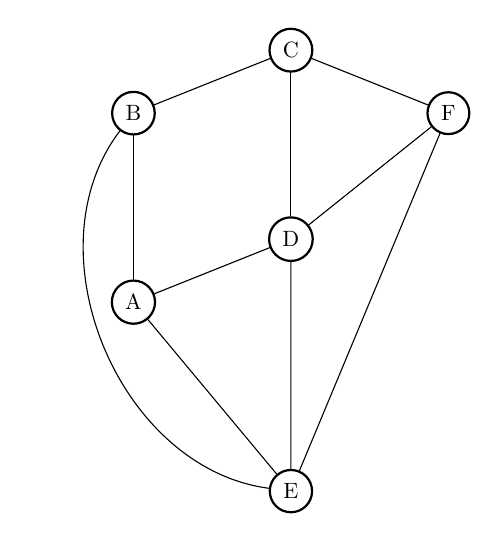
\begin{tikzpicture}[scale=0.8, transform shape]
	\begin{scope}[every node/.style={circle,thick,draw}]
		\node[] (A) at (0,0) {A};
    \node (B) at (0,3) {B};
    \node[] (C) at (2.5,4) {C};
		\node[] (D) at (2.5,1) {D};
    \node (E) at (2.5,-3) {E};
    \node (F) at (5,3) {F} ;
\end{scope}

\begin{scope}[
              every node/.style={fill=white,circle},
							every edge/.style={draw=black}]
							\path[] (A) edge[] (B);
							\path[] (B) edge[] (C);
							\path[] (A) edge[] (D);
							\path[] (D) edge[] (C);
							\path[] (A) edge[] (E);
							\path[] (D) edge (E);
							\path[] (D) edge (F);
							\path[] (C) edge[] (F);
							\path[] (E) edge (F); 
							\path[] (B) edge[bend right=60] (E); 
\end{scope}
\end{tikzpicture}
